\section{Diseño}
\label{s2:sec:Disenyo}

\subsection{Componentes del sistema}
\label{s2:subsec:sistema-entero}
A la hora de realizar el sistema, se ha decidido utilizar los siguientes
componentes:
\begin{itemize}
\item \emph{FPGA}, que como se ha comentado en la sección anterior, es la
  encargada de realizar los cálculos del juego, interpretar las órdenes de
  los usuarios, y mostrar el juego mediante un monitor VGA.
\item \emph{Maletines ARM}, encargados de leer las órdenes de los
  jugadores (mediante pulsaciones en el teclado matricial o los botones de
  la placa) y transmitirlas a la FPGA mediante una UART. Como la FPGA
  utilizada únicamente posee una UART, los maletines se pueden conectar en
  serie y transmitir los mensajes de uno hacia el siguiente hasta que
  lleguen a la FPGA (ver sección~\ref{s3:subsec:maletines}). Además, la
  FPGA transmite la información de puntuación a los maletines, los cuales
  la muestran mediante sus \emph{Display 8-Segmentos}.
\item \emph{Display 8-Segmentos}, utilizado para mostrar la información de
  puntuación.
\item \emph{Pulsadores y teclado matricial}, para que los jugadores
  indiquen sus órdenes de movimiento al sistema.
\item \emph{Monitor VGA}, utilizado para mostrar el juego.
\end{itemize}

A continuación se muestra tanto el comportamiento global del sistema, como
la comunicación entre los distintos componentes. En la sección siguiente
se muestra con más detalle el funcionamiento del componente FPGA
(apartado~\ref{s3:subsec:fpga}) y de los maletines ARM
(apartado~\ref{s3:subsec:maletines}).

\subsection{Comportamiento del sistema}
\label{s2:subsec:comportamiento}
El diseño elegido hace que el núcleo del sistema sea la FPGA, encargada del
control del juego, mientras que los maletines ARM actúan de periféricos,
modificando el estado del juego.

Esto hace que el comportamiento principal del sistema, resumido en la
figura~\ref{s2:fig:comportamiento}, consista en un bucle principal,
siguiendo los pulsos del reloj de juego, donde se va calculando el estado
actual del juego, y se reciban modificaciones externas de manera
distribuida que sirven para modificar los distintos parámetros que componen
el escenario, en este caso la posición de las raquetas de cada jugador.

Por otro lado, la FPGA notifica a los maletines el estado del juego en lo
relativo a las puntuaciones. Esta forma de abstraer el control de los
jugadores de la lógica del juego nos permitiría por ejemplo, sustituir
el control por un teclado PS2, o cualquier otro periférico, como pudiera
ser un puerto de red.

El sistema diseñado e implementado en los maletines es más sencillo
(explicado en detalle en la sección~\ref{s3:subsec:maletines}). Ambos
maletines actúan de igual manera, independientemente del orden en el que se
conecten. Los maletines envían las pulsaciones del teclado por una de las
UARTs, y en caso de recibir información por la otra, esta se trata como si
viniera de otro maletín, modificándose y reenviándose hacia la FPGA.  Este
método permite conectar en serie cualquier cantidad de maletines,
permitiendo tener un juego de N jugadores si fuese necesario\footnote{En la
  última sección~\ref{s4:sec:Conclusiones} pueden verse detalles de como
  podría convertirse en un juego de cuatro jugadores}. Además, desde el
punto de vista de la FPGA se trata de un único
maletín o teclado en el que juegan todos los jugadores de manera simultánea. \\

Este sistema podría mostrar la debilidad de un posible retardo en las
acciones realizadas por el jugador del maletín más lejano pero esto se
compensa tal y como se explica en la sección~\ref{s3:subsubsec:clocking} al llevar
diferentes relojes en cada parte del sistema; la recepción de comandos
es mucho más rápida que el reloj de movimiento del juego así que por
mucho que llegase un poco más tarde, llegaría antes del siguiente ciclo
de reloj de movimiento.

\begin{figure}[h]
  \centering
  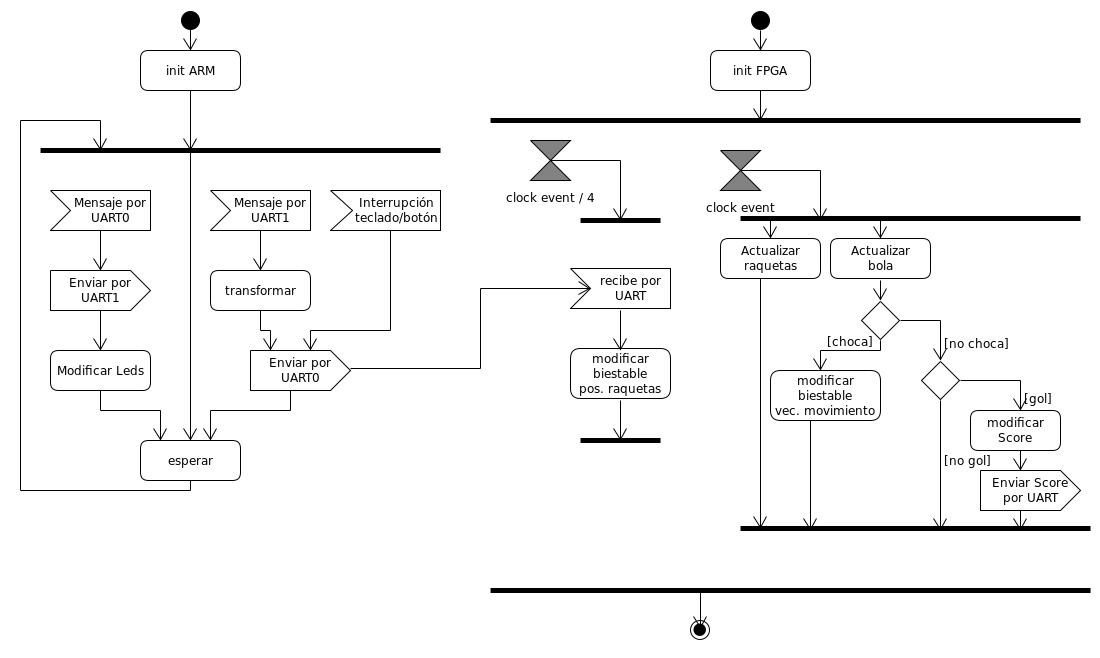
\includegraphics[width=1.0\textwidth]{images/sistema.png}
  \caption{Diagrama de Actividad del sistema (sin VGA).}
  \label{s2:fig:comportamiento}
\end{figure}

\subsection{Comunicación entre componentes}
\label{s2:subsec:comunicacion}
Como se ha mencionado anteriormente, el sistema está controlado por una
FPGA, la cual ejecuta varios bucles de manera paralela para modificar el
estado del juego y pintar en el monitor VGA los elementos del juego. El
resto de componentes (maletín, display 8-Segmentos, pulsadores, $\ldots$)
sirven para modificar el estado del juego mediante comunicaciones con la
FPGA, que permiten que esta calcule las nuevas posiciones. Según qué
componentes interactúen entre ellos, la comunicación usada es diferente:
\begin{itemize}
\item \emph{FPGA -- VGA:} Comunicación unidireccional utilizando el
  conector VGA. Se utilizan 9 líneas para los colores (3 para cada color),
  y 2 líneas adicionales para la sincronización horizontal y vertical
  respectivamente. (Más información se puede encontrar
  en~\cite{Spartan3-StarterKit}).
\item \emph{Pulsadores -- Maletín:} Detección de pulsaciones mediante
  interrupciones en la placa.
\item \emph{Maletín -- Maletín:} Comunicación mediante UARTs. El diseño
  utilizado permite conectar varios maletines en serie, por lo que el
  comportamiento general de los maletines es recibir la información por una
  UART, procesarla y reenviarla por la otra UART. Si la información es
  recibida por la UART0, se trata de otro maletín que envía información a
  la FPGA, mientras que si se recibe por la UART1, es la FPGA la que envía
  información a los maletines.
\item \emph{FPGA - Maletín:} Comunicación mediante UART. Como la FPGA
  únicamente dispone de un puerto UART, la conexión de los maletines se
  hace en serie, siendo los maletines intermedios encargados de reenviar la
  información en ambos sentidos (hacia la FPGA o hacia el resto de
  maletines).
\end{itemize}

La figura~\ref{s2:fig:secuencia} muestra de manera resumida la comunicación
entre los distintos componentes. Como se puede observar, la FPGA posee dos
grandes bucles\footnote{Más información sobre los bucles de la FPGA, y de
  manera especial sobre los distintos relojes utilizados, se puede encontrar
en~\ref{s3:subsubsec:clocking}.} encargados de calcular el estado del juego, y de pintar en
el monitor. Cuando un jugador pulsa un botón, la información es transmitida
a la FPGA a través de los maletines, modificando el cálculo del estado del
juego. En el caso de que un jugador falle, la FPGA envía información hacia
los maletines para informar de la nueva puntuación.

\begin{figure}[h]
  \centering
  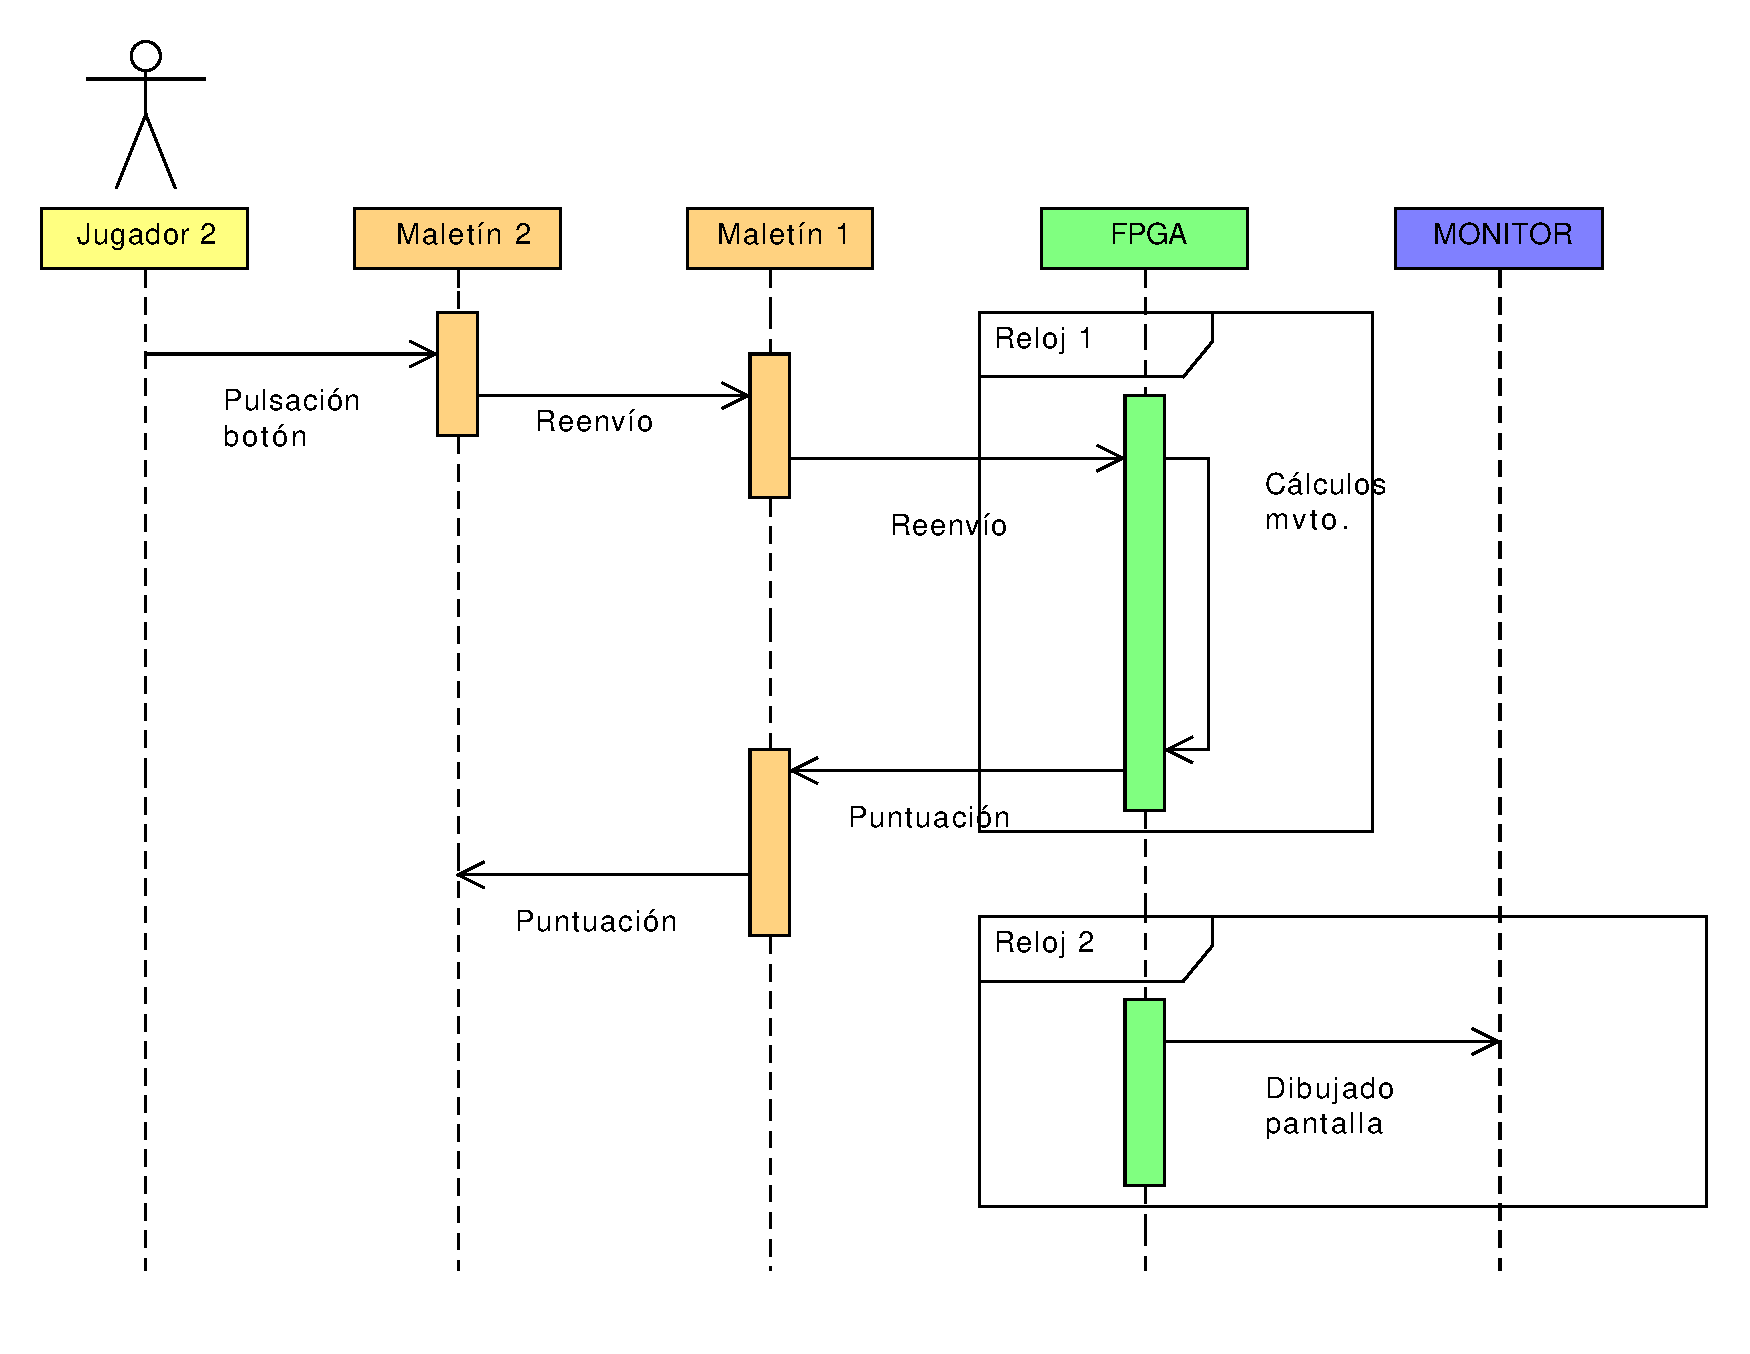
\includegraphics[width=1.0\textwidth]{images/secuencia.pdf}
  \caption{Diagrama de secuencia entre los distintos componentes.}
  \label{s2:fig:secuencia}
p\end{figure}



%
%
%%%
%%% Local Variables:
%%% mode: latex
%%% TeX-master: "../main.tex"
%%% End:


